%!TEX root = ../Hardtung_BA_SoSe20.tex

\section{Evaluating Origrammer}
\label{sec:evaluation}

To begin the evaluation process the 10 usability heuristics by Jakob Nielsen \cite{10usability_heuristics} will be used in order to facilitate a base, on which can be build upon with other evaluation methods if required. As established in \ref{sec:evaluationMethods}, the Usabilty Heuristics sometimes only identify problems without providing direct solutions. This is why this chapter will focus on finding problems and shortcomings of the Origrammer first. Afterwards, solutions can be developed that optimally fix most, or all, discovered issues without contradicting or counteracting other measures.

%Should i include Covid-19 problems in the bachelor thesis?
As the current (at the time of writing this thesis) Covid-19 pandemic hinders user involvement for the evaluation process, other measures have to be taken to ensure maximum efficiency and thoroughness. This is why there is an exhaustive list of all parts and features of the Origrammer below. Figure \ref{fig:origrammerMain} roughly shows what features are located where on the Origrammer.

\begin{figure}[htbp]
	\centering
	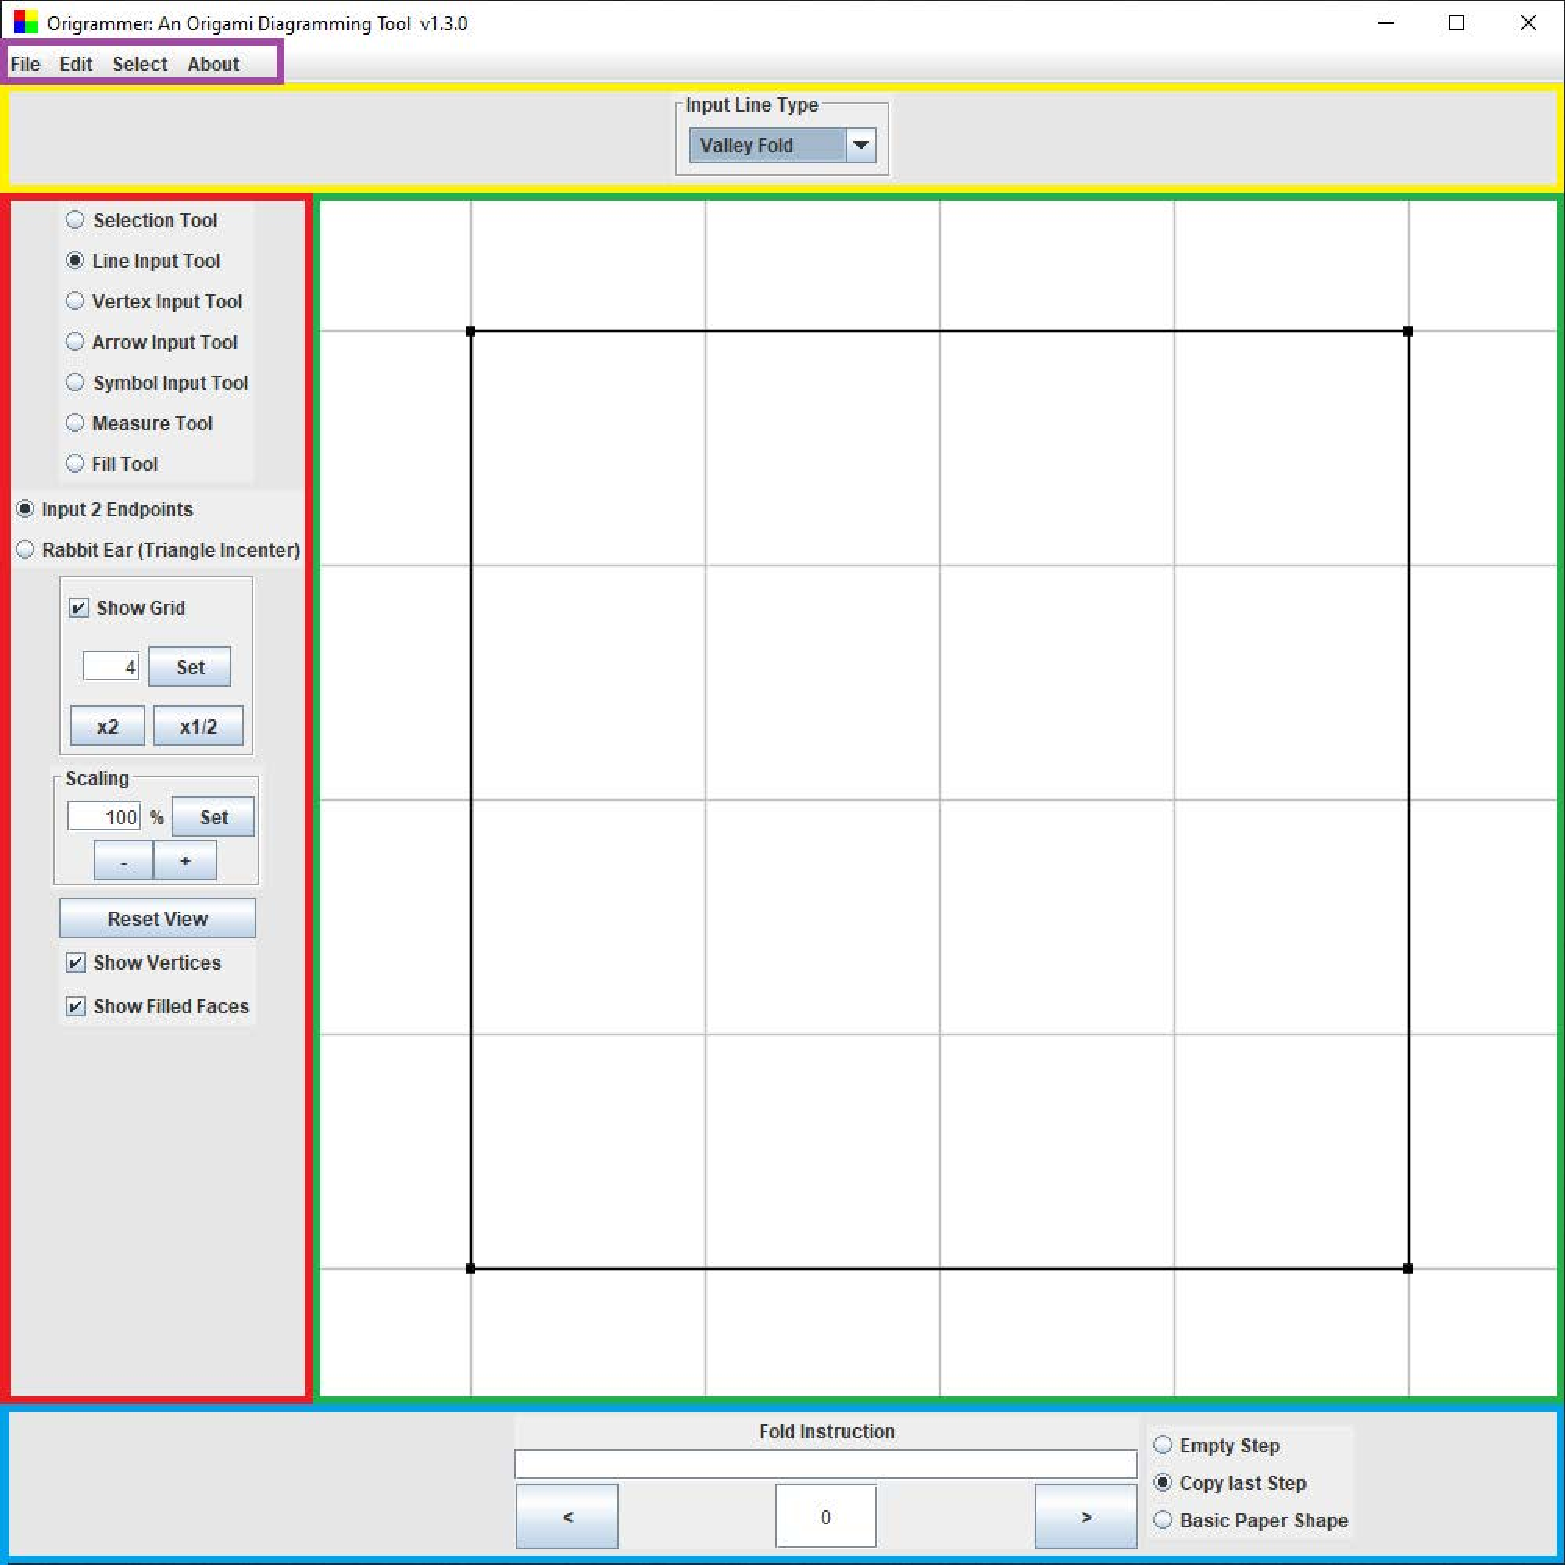
\includegraphics[width=0.8\textwidth]{OrigrammerMainParts}
	\caption{Menu Bar (Purple), Top Panel (Yellow), Side Panel (Red), Editing Panel (Green), Navigation Panel (Blue)}
	\label{fig:origrammerMain}
\end{figure}

\subsection{Origrammer Feature List}
\label{sec:featureList}

\begin{enumerate}
\item \textbf{Menu Bar (Purple)}

\begin{tabular}{l l l}
(a) New File & (b) Open File & (c) Save File \\
\emph{(d) Export File} & (e) Model Preferences & (f) Origrammer Preferences \\
\end{tabular}

\item \textbf{Side Bar (Red)}
    \begin{enumerate}
        \item Selection Tool \\
        \begin{tabular}{l l l}
        1. Click to Select & 2. Hover over Object & 3. Rectangular Selection \\
        \end{tabular}
        \item Line Input \\
        \begin{tabular}{l l}
        1. Two Point Input & 2. Triangle Incenter \\
        \end{tabular}
        \item Vertex Input \\
        \begin{tabular}{l l}
        1. Absolute Position & 2. Fraction of a Line \\
        \end{tabular}
        \item Arrow Input \\
        \begin{tabular}{l l l}
        1. Valley Fold & 2. Mountain Fold & 3. Turn over \\
        4. Push Here & 5. Pull out & 6. Inflate here \\
        \end{tabular}
        \item Symbol Input \\
        \begin{tabular}{l l l}
        1. Leader & 2. Repetition Box & 3. Next View Here \\
        4. Rotations & 5. Hold Here & 6. Hold Here and Pull \\
        7. X-Ray Circle & \emph{8. Fold Over \& Over} & 9. Equal Distances \\
        10. Equal Angles & 11. Crimps & 12. Pleats \\
        13. Closed Sinks
        \end{tabular}
        \item Measure Tool \\
        \begin{tabular}{l l l}
        1. Measure Length & 2. Measure Angle \\
        \end{tabular}
        \item Fill Tool
        \item Grid Settings
        \item Scaling Settings
    \end{enumerate}
\item \textbf{Navigation Panel (Blue)} \\
\begin{tabular}{l l l}
1. Fold Instructions & 2. Step Navigation & 3. New Step Options \\
\end{tabular}
\item \textbf{Top Panel (Yellow)} \\
See Side Panel for related features, as options for the selected Side Panel Tools appear on the Top Panel.
\item \textbf{Editing Panel (Green)} \\
See Side Panel for related features, as the selected Side Panel Tools are being used on the Editing Panel.
\end{enumerate}


\subsection{10 Usability Heuristics}
\label{sec:usabilityHeuristics}

With the Origrammer Feature List as a basis, the evalutation using the 10 Usability Heuristics can be carried out. Every feature from the list will be checked against all 10 heuristics in order to try and maximise the completeness of the result. The found usability issues will then lead to the planning of potential usability improvements.




\subsubsection*{1. Visibility of System Status}
\label{sec:visivility}

        \begin{tabular}{l | p{0.2\textwidth} | c | p{0.5\textwidth}}
        Nr: & Affects & Impact & Description \\ \hline
        01 & 2.b; 2.d-2.g & 3 & When an action requires multiple input points (e.g. placing a Fold Line by two endpoints), the user doesn't know where he is in the process. \\ \hline %maybe progressbar 
        02 & 1.1-1.6; 2.b-2.i; 3.1-3.3 & 3 & When an action requires multiple steps, 
        \end{tabular}



\subsubsection*{2. Aesthetic and Minimalist Design}
        \begin{tabular}{l | p{0.2\textwidth} | c | p{0.5\textwidth}}
        Nr: & Affects & Impact & Description \\ \hline
        02 & 2.a-2.i; 4;  & 3 &  Redundant information should be removed and/or replaced by Symbols or Icons (e.g. the Tool Selection on the SidePanel can be replaced by icons)\\ \hline 


        \end{tabular}

\subsubsection*{3. User Control and Freedom}

User should always be able to cancel an action (like placing symbol)

\subsubsection*{4. Consistency and Standards}

Editing of symbols/arrows should be correctly labeled

When selecting and editing Symbols/arrows make it consistent (don't let multiple different symbols be selected at the same time

\subsubsection*{5. Error Prevention}

Prevent impossible and breaking user inputs

\subsubsection*{6. Recognition Rather than Recall}

Don't make the user remember stuff (only keyboard shortcuts)

\subsubsection*{7. Flexibility and Efficiency of Use}

\subsubsection*{8. Recognition, Diagnosis and Recovery from Errors}

\subsubsection*{9. Help and Documentation}

Show tooltips when hovering over stuff

Show short explanation when using a feature (bottom left --> see \ref{visibility}

\subsubsection*{10. Match between System and Real World}